%% Source: https://github.com/tias/constraint-solving-course
%% Licensed under CC BY-NC-SA 4.0: https://creativecommons.org/licenses/by-nc-sa/4.0/
%% You may share and adapt this for non-commercial use,
%% with attribution and under the same license.

\documentclass{cons-beamer}

\begin{document}


\begin{frame}{L04: Global Constraints}
  \begin{center}
    ~ \\
    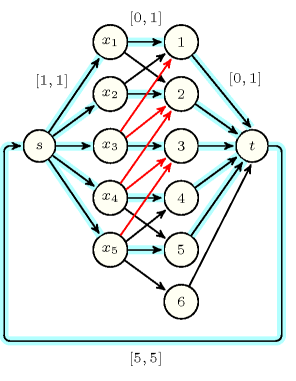
\includegraphics[height=42mm]{images/flow_alldiff_only_graph.png} \\
    Prof. Tias Guns and Dr. Dimos Tsouros \\[0.5em]
    
\includegraphics[width=2cm]{images/kuleuven_CMYK_logo.pdf}
  \end{center}
  
  {\footnotesize 
  Partly based on slides from Pierre Flener, Uppsala University.}
  % https://pierre-flener.github.io/courses/M4CO/lectures.html
\end{frame}


\section{Definition}

\begin{frame}
  \begin{definition}
    \textit{Global Constraint}: an expressive and concise constraint that  
    \begin{itemize}
      \item is defined over a non-fixed number of variables,
      \item captures a specific combinatorial substructure commonly found in constraint satisfaction problems   
    \end{itemize}
  \end{definition} \vfill

  \begin{example}
    Well-known global constraints
    \begin{itemize}
      \item \cons{AllDifferent}{}
      \item \cons{Circuit}{}
      \item \cons{Cumulative}{}
      \item \dots
    \end{itemize}
  \end{example}
\end{frame}


\section{Motivation}

\begin{frame}{Why use Global Constraints?} 
  \begin{itemize}
    \item[+] \textbf{Expressiveness}! \\ 
      More compact and intuitive models, closer to problem definition \\ 
      Many expressive predicates are available: \\
      islands of common combinatorial structure are identified in declarative high-level abstractions. \\
      See the \href{https://sofdem.github.io/gccat}{Global-Constraint Catalogue}.
      \vfill 

    \item[+] \textbf{Efficiency}! (In CP solvers) \\
      Faster solving, \\
      due to better \inference{inference} and \relaxation{relaxation}, \\
      enabled by more global information in the model \\
      (If supported by the used solver.)
  \end{itemize}
\end{frame}

\begin{frame}{Why use Global Constraints?}
  \begin{itemize}
    \item[+] \textbf{Expressiveness}! \\
      More compact and intuitive models, closer to problem definition. \\ 
      Many expressive global constraints available \vfill 
      \begin{itemize}
        \item \textbf{Simplified modeling}: Global constraints enable the modeler to express complex conditions simpler. \\
              Simpler modeling reduces the chance of modeling errors.

        \item \textbf{Compactness}: Instead of writing multiple smaller constraints, a single global constraint can capture the entire logic. \\
Make the model more intuitive and readable
      \end{itemize}
  \end{itemize}
  \vfill

  \begin{example}
    Task allocation: I want all tasks to be allocated to a different team. \\
    \begin{itemize}
      \item \textit{Without global}: \\
            $Task_0 \neq Task_1, \; Task_0 \neq Task_2, \; Task_1 \neq Task_2, \; \dots$
      \item \textit{With global}: \cons{AllDifferent}{Task}
    \end{itemize}
  \end{example}
\end{frame}

\begin{flashcardcpmpy}
\begin{frame}{Why use Global Constraints? -- CPMpy}
  \begin{itemize}
    \item[+] \textbf{Expressiveness}! \\ More compact and intuitive models, closer to problem definition. \\ 
             Many expressive global constraints available \vfill
             \begin{itemize}
                \item \textbf{Simplified modeling}: Global constraints enable the modeler to express complex conditions simpler. \\
                      Simpler modeling reduces the chance of modeling errors.

                \item \textbf{Compactness}:  Instead of writing multiple smaller constraints, a single global constraint can capture the entire logic. \\
                      Make the model more intuitive and readable
             \end{itemize}
  \end{itemize}
  \vfill

  \begin{example}
    Task allocation: I want all tasks to be allocated to a different team\\
    \begin{itemize}
      \item \textit{Without global}: \\ \cpminline{Task[0] != Task[1], Task[0] != Task[2], Task[1] != Task[2],} \dots \\
      \item \textit{With global}:  \cpminline{cp.AllDifferent(Task)}
    \end{itemize}
  \end{example}
\end{frame}
\end{flashcardcpmpy}

\begin{frame}{Why use Global Constraints?}
  \begin{itemize}
    \item[+] \textbf{Efficiency}! (In CP solvers) \\ Faster solving, due to better \inference{inference} and
             \relaxation{relaxation}, enabled by more global information in
             the model (If supported by the used solver.)
             \begin{itemize}
               \item More global information in one constraint can result to advanced filtering of the \search{search} space
               \item Specialized algorithms to detect \conflict{conflicts} faster during solving.
             \end{itemize}
  \end{itemize}
  \vfill

  \begin{example}
    \textbf{Task allocation}: I want to allocate $n$ tasks to $m$ teams, s.t. each task is assigned to a different team. Assume we have $m < n$. \\
    \begin{itemize}
      \item \textit{Without global}: Each $!=$ constraint needs 2 values (teams) available for its tasks. Will realize that there are not enough values only after extensive search of possible assignments \\
      \item \textit{With global}: \cons{AllDifferent}{Task} will directly recognise that we cannot put $m$ different values (teams) in $n$ variables (tasks) if we have $m < n$ during search. $\leftarrow$ \textbf{Pigeonhole principle}
    \end{itemize}
  \end{example}
\end{frame}

\begin{frame}{Modelling with Global Constraints:}
  \vfill
  
  Several global constraints exist, capturing different combinatorial properties: \\
  Global-Constraint Catalogue \url{https://sofdem.github.io/gccat}
  \vfill

  \textbf{Functional Global Constraints}: Global constraints that have a functional component, such as \cons{MinimumEq}{}, \cons{MaximumEq}{}, \cons{CountEq}{}, \cons{NValueEq}{}, etc.
  \vfill

  \begin{definition}
    A global constraint \cons{G}{V} is functional if and only if there exists a partitioning of the arguments $V$ of the constraint into two non-empty and non-overlapping subsets $V1, V2$, such that \textit{the assignment of variables in subset $V2$ is defined using a function on the subset $V1$}.
  \end{definition}
\end{frame}

\begin{frame}{Modelling with Global Constraints:}
  \vfill

  \begin{definition}
    A global constraint \cons{G}{V} is functional if and only if there exists a partitioning of the arguments $V$ of the constraint into two non-empty and non-overlapping subsets $V1, V2$, such that \textit{the assignment of variables in subset $V2$ is defined using a function on the subset $V1$}.
  \end{definition}
  \vfill

  In many cases, this involves associating the value of the functional component with a variable:

  \begin{examples}
    \begin{itemize}
      \item \cons{MaximumEq}{X, v} implies that \cons{Maximum}{X} $= v$, allowing $v$ to be used in other expressions.
      \item \cons{MinimumEq}{X, v} implies that \cons{Maximum}{X} $= v$, allowing $v$ to be used in other expressions.
      \item \dots
    \end{itemize}
  \end{examples} 
\end{frame}

\begin{flashcardcpmpy}
\begin{frame}{Modelling with Global Constraints -- CPMpy}
  \begin{itemize}
    \item Several commonly-used global constraints are available: \\ \cpminline{AllDifferent, AllEqual, Cumulative, Table,} \dots
      \begin{footnotesize}
        API documentation: \\ \url{http://cpmpy.readthedocs.io/en/latest/api/expressions/globalconstraints.html}
      \end{footnotesize} \vfill
    \item \textbf{Functional Global Constraints}: A subset of them, the ones associating the result of a function to a variable, are modelled as 'Global functions' in \CPMpy, representing only the \textit{functional} component: e.g. \cpminline{cp.Count(X,1)}
    \begin{itemize}
      \item Can be used nested in any expression: e.g. \cpminline{cp.Count(X,1) > 0}
      \item Several Global functions available: \\ \cpminline{Minimum, Maximum, Count, NValue,} \dots 
        \begin{footnotesize}
          API documentation: \\ \url{http://cpmpy.readthedocs.io/en/latest/api/expressions/globalfunctions.html}
        \end{footnotesize}
    \end{itemize} \vfill
    \item All global constraints can be reified - be nested in other expressions: e.g. \\
      \cpminline{cp.sum(cp.AllDifferent(x), cp.AllDifferent(y), cp.AllDifferent(z)) > 2} \vfill
    \item Can use globals that the chosen solver might not support. CPMpy will translate this to a lower-level solver decomposition for you.
  \end{itemize}
\end{frame}
\end{flashcardcpmpy}

\section{Common Global Constraints}

\subsection{\cons{AllDifferent}{}}

\begin{frame}{\cons{AllDifferent}{}}
  \begin{definition}[Lauri\`ere, 1978]
    The \cons{AllDifferent}{X} constraint holds if and only if all the elements of the array $X$ of decision variables take distinct values.
  \end{definition}
  
  Its decomposition is a conjunction of \(\frac{n \cdot (n-1)}{2}\) disequality constraints \\
  when \( X \) has \( n \) elements:
  \[
  \forall i, j \in \{1, \ldots, n\}, i < j \implies X[i] \neq X[j]
  \]
  \vfill

  \begin{examples}
    \begin{itemize}
      \item $n$-Queens, Photo Alignment problem, Student Seating problem.
      \item Sudoku, Room assignment, Task allocation \dots
    \end{itemize}
  \end{examples}
  \vfill

  Variant: The \cons{AllDifferentExceptN}{X, N} constraint allows multiple occurrences of the exception values in the set \( N \).
\end{frame}

\begin{flashcardcpmpy}
\begin{frame}{\cons{AllDifferent}{} -- CPMpy}
  \begin{definition}[Lauri\`ere, 1978]
    The \cons{AllDifferent}{X} constraint holds if and only if all the elements of the array $X$ of decision variables take distinct values.
  \end{definition}
  Its decomposition is a conjunction of \(\frac{n \cdot (n-1)}{2}\) disequality constraints \\
  when \( X \) has \( n \) elements:
  \begin{center}
    \cpminline{[var1 != var2 for var1, var2 in all_pairs(X)]}
  \end{center}
  \vfill
  
  \begin{examples}
    \begin{itemize}
      \item $n$-Queens, Photo Alignment problem, Student Seating problem.
      \item Sudoku, Room assignment, Task allocation \dots
    \end{itemize}
  \end{examples}
  \vfill

  Variant: The \cons{AllDifferentExceptN}{X, N} constraint allows multiple occurrences of the exception values in the set \( N \).
\end{frame}
\end{flashcardcpmpy}

\begin{frame}
  \begin{example}
    Sudoku: we want different values in rows, columns and blocks \\
    using the \cons{AllDifferent}{X} global constraint 
    \begin{align*}
      &\text{AllDifferent}(\{G_{ij} \mid j \in \{1, \ldots, 9\}\}) & & \forall i \in \{1, \ldots, 9\} \quad \text{(rows)} \\
      &\text{AllDifferent}(\{G_{ij} \mid i \in \{1, \ldots, 9\}\}) & & \forall j \in \{1, \ldots, 9\} \quad \text{(columns)} \\
      &\text{AllDifferent}(\{G_{kl} \mid k \in \{i, \ldots, i+2\}, l \in \{j, \ldots, j+2\}\}) & & \forall i, j \in \{1, 4, 7\} \quad \text{(blocks)}
    \end{align*}

    Way more expressive (and efficient) than using binary not equal constraints
    
    \begin{align*}
      &G_{ij} \neq G_{ik} & \quad & \forall i \in \{1, \ldots, 9\}, \, \forall j, k \in \{1, \ldots, 9\}, \, j < k \quad \text{(rows)} \\
      &G_{ij} \neq G_{kj} & \quad & \forall j \in \{1, \ldots, 9\}, \, \forall i, k \in \{1, \ldots, 9\}, \, i < k \quad \text{(columns)} \\
      &G_{kl} \neq G_{mn} & \quad & \forall i, j \in \{1, 4, 7\}, \ \forall k, m \in \{i, \ldots, i+2\}, \\
      & & & \, \forall l, n \in \{j, \ldots, j+2\}, \, (k, l) < (m, n) \quad \text{(blocks)}
    \end{align*}
  \end{example}
\end{frame}

\begin{flashcardcpmpy}
\begin{frame}
  \begin{example}[CPMpy]
    Sudoku: we want different values in rows, columns and blocks

    \lstinputlisting[language=cpmpy,basicstyle=\small,firstline=21,lastline=24]{models_cpmpy/T01_sudoku.py}
    \vfill

    Way more efficient solving than when using binary not equal constraints
    \vfill

    \lstinputlisting[language=cpmpy,basicstyle=\small,firstline=24,lastline=30]{models_cpmpy/sudoku_binary.py}
  \end{example}
\end{frame}
\end{flashcardcpmpy}

\begin{frame}
  \begin{itemize}
    \item[+] \textbf{Efficiency}! Better propagation in CP solvers due to capturing global properties \\ 
  \end{itemize}
  \vfill
  \begin{columns}
    \begin{column}{0.3\textwidth}
      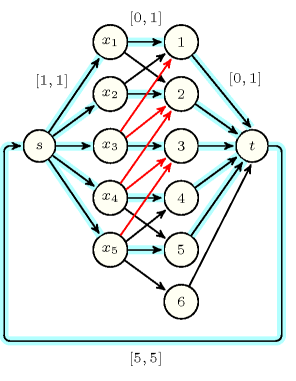
\includegraphics[width=45mm]{images/flow_alldiff_only_graph.png} \\
    \end{column}
    \begin{column}{0.7\textwidth}
      Flow model for the \cons{AllDifferent}{} constraint
      \begin{itemize}
        \item feasible flows in the flow model = solutions to the constraint \vfill
        \item detect arcs that cannot carry flow in any feasible solutions $\rightarrow$ \inference{remove values from the domains of variables} \vfill
        \item \blue{Blue} arcs represent feasible flows, \red{red} arcs represent infeasible ones \vfill
        \item \textbf{Detect inconsistency early}: flow from (some) variables \red{cannot} be directed through the available values $\rightarrow$ pigeonhole problem
        \begin{itemize}
          \item Not detected early through binary constraints \vfill
        \end{itemize}
      \end{itemize}
    \end{column}
  \end{columns}
\end{frame}


\subsection{\cons{GlobalCardinalityCount}{}}    

\begin{frame}{\cons{GlobalCardinalityCount}{}}
  \begin{definition}[R\'{e}gin, 1996]
    The \cons{GlobalCardinalityCount}{X, V, C} constraint holds if and only if the number of occurrences of each value \( V_i \) in the list of variables \( X \) is equal to \( C_i \).
  \end{definition}
  \vfill

  Its decomposition is expressed as:
  \[
  \forall j \in \{1, \ldots, |V|\}, \quad \text{CountEq}(X, V_j, C_j) 
  \]
  which is: 
  \[
  \sum_{i}  [ X_i = V_j ]  = C_j
  \]
  \vfill

  This constraint is equivalent to \cons{AllDifferent}{X} if:
  \[
  V = \bigcup_{i} \text{Domain}(X_i) \quad \text{and} \quad \text{Domain}(C_j) = \{0, 1\} \quad \forall j
  \]
  
  However, always use the most specific available constraint predicate!
\end{frame}

\begin{flashcardcpmpy}
\begin{frame}{\cons{GlobalCardinalityCount}{} -- CPMpy}
  \begin{definition}[R\'{e}gin, 1996]
    The \cons{GlobalCardinalityCount}{X, V, C} constraint holds if and only if the number of occurrences of each value \( V[i] \) in the list of variables \( X \) is equal to \( C[i] \).
  \end{definition}
  \vfill

  Its decomposition in \CPMpy is:
  
  \cpminline{[cp.Count(X, v) == c for v, c in zip(V, c)]} 
  
  Add \blue{\cpminline{closed=True}} as a parameter if
  \cpminline{V} must be forced as the domain of the variables in \cpminline{X}.
  \vfill

  This constraint is equivalent to \cons{AllDifferent}{X} if:
  \[
  V = \bigcup_{i} \text{Domain}(X[i]) \quad \text{and} \quad \text{Domain}(C[j]) = \{0, 1\} \quad \forall j
  \]

  However, always use the most specific available constraint predicate!
\end{frame}
\end{flashcardcpmpy}
\begin{flashcardminizinc}
\begin{frame}[fragile]%{The \mzninline{global_cardinality} Predicate}
  \begin{definition}[R\'{e}gin, 1996]
    The \uppsala{\mzninline{global_cardinality(X,V,C)} constraint holds if and
    only if each decision variable \mzninline{C[j]} takes the number
    of elements of the array \mzninline{X} of decision variables that
    take the given \emph{value}~ \mzninline{V[j]}.
    %
    Variant predicates exist. \\
    %
    Add \blue{\mzninline{_closed}} to the predicate name if
    \mzninline{V} is the domain of the variables in \mzninline{X}.}
    \kuleuven{\cpminline{GlobalCardinalityCount(X,V,C)}} global constraint holds if and only if The number of occurrences of each value \cpminline{V[i]} in the list of variables \cpminline{X}
    is equal to \cpminline{C[i]}.
    \end{definition} \vfill

    \kuleuven{Its decomposition in \CPMpy is:
    \cpminline{[Count(X, v) == c for v, c in zip(V, c)]} \\
    Add \blue{\cpminline{closed=True}} as a parameter if
    \cpminline{V} must be forced as the domain of the variables in \cpminline{X}.}
  \vfill
  
  Equivalent to \uppsala{\mzninline{all_different(X)}} \kuleuven{\cpminline{AllDifferent(X)}} if 
  \uppsala{$\mzninline{V} = \bigcup_{\mzninline{i}} \Domain{\mzninline{X[i]}}$
  and~$\Domain{\mzninline{C[j]}} = \Set{0,1}$ for each \mzninline{j},}
  \kuleuven{$V = \bigcup_{i} \Domain{X[i]}$
  and $\Domain{C[j]} = \Set{0,1}$ for each \cpminline{j},}
   but: \alert{Always use the most specific available constraint
    predicate!}  \vfill
\end{frame}
\end{flashcardminizinc}

\begin{frame}{Facility Location}
  \vspace{-1.5em}
  \begin{columns}
    \begin{column}{0.6\textwidth}
      Warehouse location: we want to find which customers each warehouse will serve
    \end{column}
    \begin{column}{0.4\textwidth}
      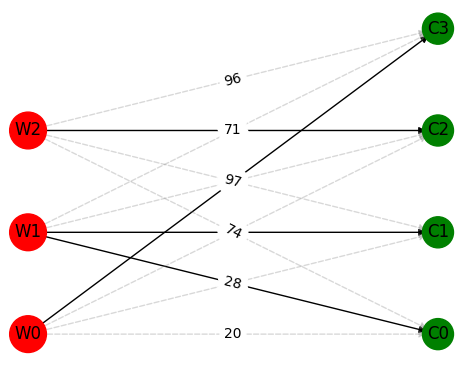
\includegraphics[width=40mm]{images/warehouse_plot.png} \\
    \end{column}
  \end{columns}

  \begin{example}
    \vfill
    Use the \cons{GlobalCardinalityCount}{assignments, warehouses, capacities} constraint to ensure that each warehouse is assigned the correct number of customers.
    \vfill
  \end{example}

  \alert{\cons{GlobalCardinalityCount}{} defines the exact number of occurencies, not a bound, i.e. takes capacity for each variable} \\ \vfill

  \blue{But every argument can be a variable! So, you can use variables (with the specified bounds) as capacities} \\ \vfill
  \vfill
\end{frame}

\begin{flashcardcpmpy}
\begin{frame}{Facility Location -- CPMpy}
  \vspace{-1.5em}
  \begin{columns}
    \begin{column}{0.6\textwidth}
      Warehouse location: we want to find which customers each warehouse will serve
    \end{column}
    \begin{column}{0.4\textwidth}
      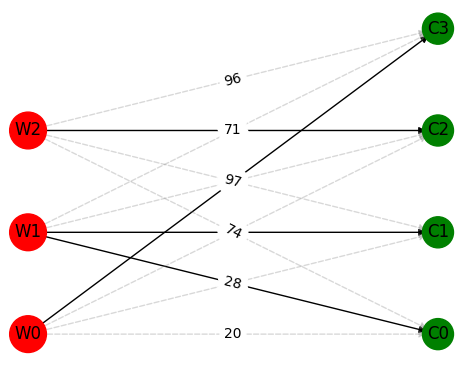
\includegraphics[width=40mm]{images/warehouse_plot.png} \\
    \end{column}
  \end{columns}

  \begin{example}[CPMpy]
    \vspace{-0.5em}
    \footnotesize
    \lstinputlisting[language=cpmpy,basicstyle=\small,firstline=13,lastline=14]{models_cpmpy/t4_gcc.py}
    \vspace{-0.5em}
  \end{example}

  \alert{\cons{GlobalCardinalityCount}{} defines the exact nr of occurencies, not a bound} \\ \vfill
  \blue{But every argument can be a variable! So, you can use variables (with the specified bounds) as capacities} \\ \vfill 
  But, why not model it directly using \cpminline{cp.Count}? 
  We will discuss this later!  
\end{frame}
\end{flashcardcpmpy}


\subsection{Scheduling with \cons{Cumulative}{} and \cons{NoOverlap}{}}

\begin{frame}{Scheduling}
  Assume we need to schedule a set of non-interruptible tasks
  % that are to be performed over a given period
  under constraints (on resources, precedences, \dots) such that the
  last task has the earliest end.
  \begin{definition}
    A task $T_i$ is defined as a triple of parameters $ T_i = \langle S_i, D_i, R_i \rangle$ or
    % decision
    variables, where:
    \begin{itemize}
      \item $S_i$ is the starting time of task $T_{\mzninline{i}}$
      \item $D_i$ is the duration of task $T_{\mzninline{i}}$
      \item $R_i$ is the quantity of a global reusable
        resource needed by $T_i$
    \end{itemize}
    Tasks may be run in parallel when the capacity of the global
    resource suffices.
  \end{definition}
  \vfill
  \begin{center}
    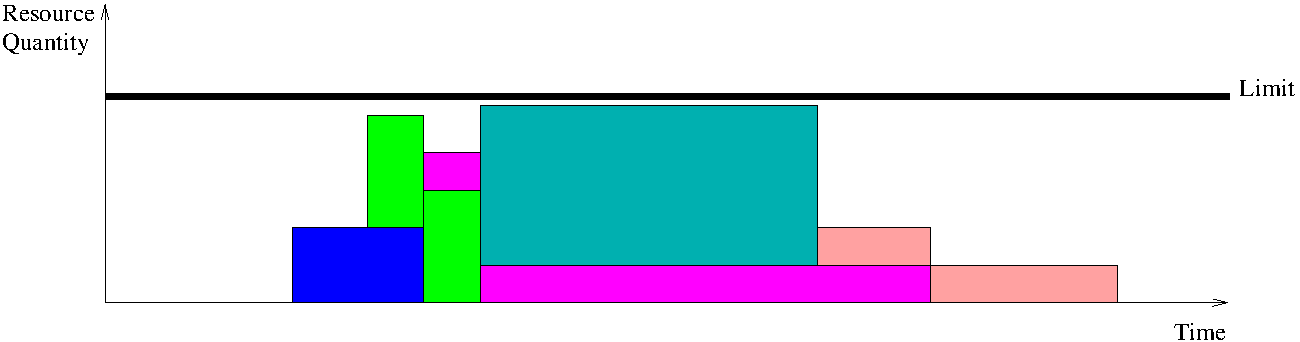
\includegraphics[width=100mm]{images/scheduling1} \\
    Schedule with parallel tasks and a capacitated global reusable resource
  \end{center}
\end{frame}

\begin{frame}\label{ex:prec}
  \begin{definition}
    A \defined{precedence constraint} of task $T_1$ on task $T_2$
    requires \\ that~$T_1$ ends \alert{before} $T_2$ starts.  We say
    that task~$T_1$ \defined{precedes} task~$T_2$.
  \end{definition}
  \vfill

  \begin{example}[courtesy Magnus Rattfeldt]
    \begin{center}
      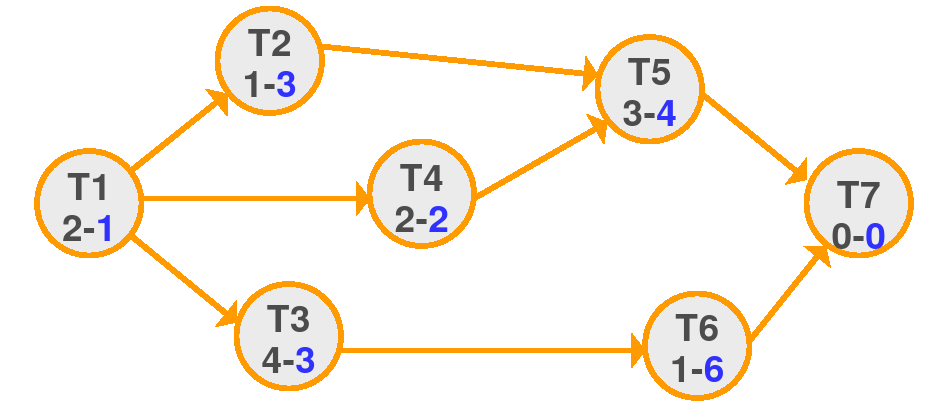
\includegraphics[width=80mm]{images/scheduling2} \\
      Sample tasks (circles), durations (black numbers), resource
      requirements (\blue{blue} numbers), and precedences
      (\textcolor{Orange}{orange} arrows).  Task~T7 is a dummy task,
      as we do not know which of tasks T5 and T6 will end last.
    \end{center}
  \end{example}
\end{frame}

\begin{frame}%{Scheduling precedences}
  Let us temporarily \textbf{ ignore the capacitated global reusable resource}: \\
  If we have an uncapacitated global reusable resource or each task
  has enough of its own local reusable resource, then the
  (polynomial-time-solvable problem) of \textbf{finding the earliest ending
  time, under only the precedence constraints}, for performing all the
  tasks can be modelled using linear inequalities.
  \vfill

  \begin{example}[continued]
    The precedence constraints indicated by the
    \textcolor{Orange}{orange} arrows on slide~\ref{ex:prec} are
    modelled as follows, based on the task durations indicated there
    in black: 

    \begin{align*}
      S_0 + D_0 \leq S_1, \quad S_0 + D_0 \leq S_2, \\ S_0 + D_0 \leq S_3, \quad S_1 + D_1 \leq S_4, \\ S_2 + D_2 \leq S_5, \quad S_3 + D_3 \leq S_4, \\ S_4 + D_4 \leq S_6, \quad S_5 + D_5 \leq S_6 \\
      \text{Minimize } S_6
    \end{align*} 
  \end{example}
\end{frame}

\begin{flashcardcpmpy}
\begin{frame}%{Scheduling precedences -- CPMpy}
  Let us temporarily \textbf{ ignore the capacitated global reusable resource}: \\
  If we have an uncapacitated global reusable resource or each task
  has enough of its own local reusable resource, then the
  (polynomial-time-solvable problem) of \textbf{finding the earliest ending
  time, under only the precedence constraints}, for performing all the
  tasks can be modelled using linear inequalities.
  \vfill

  \begin{example}[continued]
    The precedence constraints indicated by the
    \textcolor{Orange}{orange} arrows on slide~\ref{ex:prec} are
    modelled as follows, based on the task durations indicated there
    in black: 
    
    \lstinputlisting[language=cpmpy,basicstyle=\small,firstline=8,lastline=13]{models_cpmpy/t4_precedence.py}
  \end{example}
\end{frame}
\end{flashcardcpmpy}
\begin{flashcardminizinc}
\begin{frame}[fragile]%{Scheduling precedences -- MiniZinc}
  Let us temporarily \textbf{ ignore the capacitated global reusable resource}: \\
  If we have an uncapacitated global reusable resource or each task
  has enough of its own local reusable resource, then the
  (polynomial-time-solvable problem) of \textbf{finding the earliest ending
  time, under only the precedence constraints}, for performing all the
  tasks can be modelled using linear inequalities.
  \vfill

  \begin{example}[continued]
    The precedence constraints indicated by the
    \textcolor{Orange}{orange} arrows on slide~\ref{ex:prec} are
    modelled as follows, based on the task durations indicated there
    in black: 
    
    \begin{mzn}
constraint D = [2,1,4,2,3,1,0];
constraint S[1]+D[1] <= S[2] /\ S[1]+D[1] <= S[3]
        /\ S[1]+D[1] <= S[4] /\ S[2]+D[2] <= S[5]
        /\ S[3]+D[3] <= S[6] /\ S[4]+D[4] <= S[5]
        /\ S[5]+D[5] <= S[7] /\ S[6]+D[6] <= S[7];
% plug in here the resource constraint of the next slide
solve minimize S[7];
    \end{mzn}
  \end{example}
\end{frame}
\end{flashcardminizinc}

\begin{frame}{But how to model the capacitated global resource?}
  \begin{definition}[Aggoun and Beldiceanu, 1993]
    The \cons{Cumulative}{S, D, R, c} constraint, for tasks \( T_i = \langle S_i, D_i, R_i \rangle \),
    holds if and only if the total resource usage does not exceed the capacity \( c \) at any time.
  \end{definition}
  \vfill

  The \cons{Cumulative}{S, D, R, c} ensures the following:
  \[
  \sum_{i: S_i \leq t < S_i + D_i} R_i \leq c, \quad \forall t
  \]
  \vfill

  Note that \cons{Cumulative}{S, D, R, c} does \alert{not} ensure any
  precedence constraints between the tasks: \\these have to be stated
  separately (as on the previous slide). 
\end{frame}

\begin{frame}
  \begin{center}
    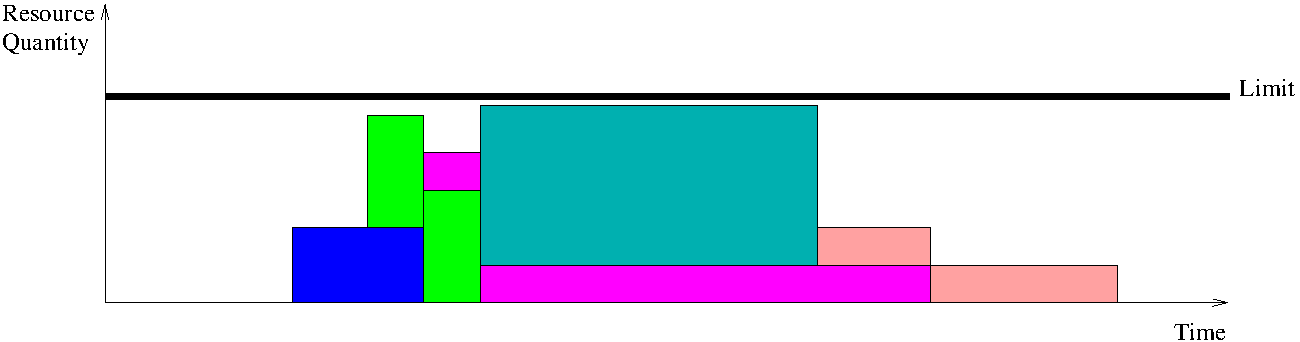
\includegraphics[width=75mm]{images/scheduling1}
  \end{center}
  
  \begin{example}[Cumulative]
    To ensure that the global reusable resource capacity of
    $c = 8$ units, say, is never exceeded under the resource
    requirements of the tasks indicated in \blue{blue} on
    slide~\ref{ex:prec}, use the following constraint: 

    \cons{Cumulative}{S, D, [1, 3, 3, 2, 4, 6, 0], 8}
    
    Along with the precedence constraints described before:
    \begin{align*}
      S_0 + D_0 \leq S_1, \quad S_0 + D_0 \leq S_2, \quad S_0 + D_0 \leq S_3, \quad S_1 + D_1 \leq S_4, \\ S_2 + D_2 \leq S_5, \quad S_3 + D_3 \leq S_4, \quad S_4 + D_4 \leq S_6, \quad S_5 + D_5 \leq S_6 \\
      \text{Minimize } S_6 
    \end{align*} 
  \end{example}
\end{frame}

\begin{flashcardcpmpy}
\begin{frame}[fragile]  % [fragile] for \cpminline
  \begin{center}
    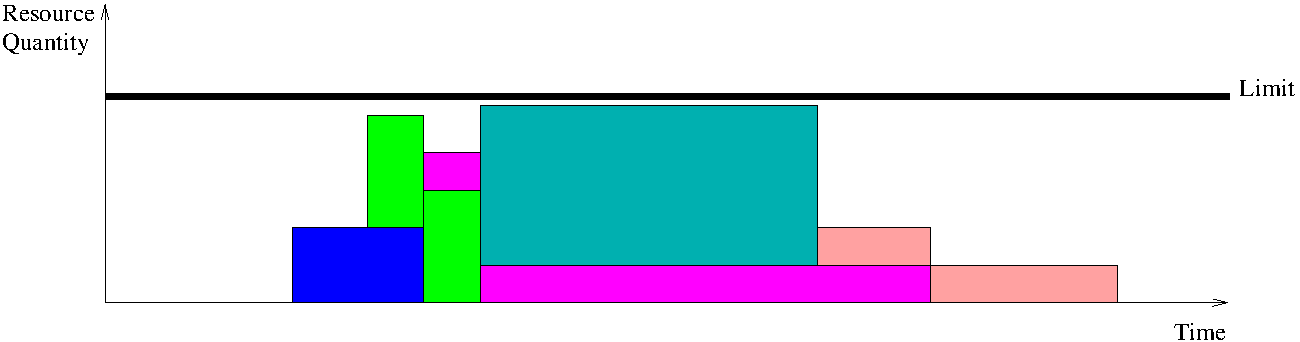
\includegraphics[width=75mm]{images/scheduling1}
  \end{center}
  
  \begin{example}[Cumulative -- CPMpy]
    To ensure that the global reusable resource capacity of
    \cpminline{c = 8} units, say, is never exceeded under the resource
    requirements of the tasks indicated in \blue{blue} on
    slide~\ref{ex:prec}, use the following constraint:
    
    \vfill
    \cpminline{# Need to define variables for E: end time of tasks!}
    \cpminline{model += cp.Cumulative(S,D,E,[1,3,3,2,4,6,0],8)}
    \vfill

    $ $
    
    Along with the precedence constraints described before:

    \lstinputlisting[language=cpmpy,basicstyle=\scriptsize,numbers=none,firstline=8,lastline=13]{models_cpmpy/t4_precedence.py}
  \end{example}
\end{frame}
\end{flashcardcpmpy}

\begin{frame}{Scheduling -- NoOverlap}
  What if I just want tasks scheduled to not overlap?
    
  A \defined{non-overlap constraint} between tasks~$T_1$ and~$T_2$
  requires that \alert{either}~$T_1$ precedes~$T_2$
  \alert{or}~$T_2$ precedes~$T_1$.
  
  \begin{definition}[Carlier, 1982]
    The \cons{NoOverlap}{S, D} constraint, where each task
    $T_i$ has the starting time $S_i$ and
    duration $D_i$, holds if and only if no two tasks $T_i$ and $T_j$ overlap in time.
  \end{definition}

  Its decomposition is:
  \begin{align*}
    & S_i + D_i \leq S_j \quad \text{or} \quad S_j + D_j \leq S_i \quad \forall i, j \text{ with } i \neq j
  \end{align*}
  \vfill

  Can be also modeled as: \cons{Cumulative}{S, D, [1, 1, \ldots, 1], 1}

  \alert{Always use the most specific available constraint predicate!}
\end{frame}

\begin{flashcardcpmpy}
\begin{frame}{Scheduling -- NoOverlap -- CPMpy}
  What if I just want tasks scheduled to not overlap?
    
  A \defined{non-overlap constraint} between tasks~$T_1$ and~$T_2$
  requires that \alert{either}~$T_1$ precedes~$T_2$
  \alert{or}~$T_2$ precedes~$T_1$.
  
  \begin{definition}[Carlier, 1982]
    The \cons{NoOverlap}{S, D} constraint, where each task
    $T_i$ has the starting time $S_i$ and
    duration $D_i$, holds if and only if no two tasks $T_i$ and $T_j$ overlap in time.
  \end{definition}

  In \CPMpy \cpminline{cp.NoOverlap(S,D,E)} also needs an argument for the end times of the tasks!

  $ $

  Its decomposition in \CPMpy is:
  \begin{itemize}
    \item \cpminline{for i in range(n):} \\
      ~~ \cpminline{model += S[i] + D[i] == E[i]}
    \item \cpminline{for i,j in all_pairs(range(n)):} \\
      ~~ \cpminline{model += (E[i] <= S[j]) | (E[j] <= S[i])}
  \end{itemize}
  \vfill
    
  Can be also modeled as: \cpminline{cp.Cumulative(S, D, E, [1 for i in range(n)], 1)}
    
  \alert{Always use the most specific available constraint predicate!}
\end{frame}
\end{flashcardcpmpy}


\subsection{\cons{Circuit}{}}

\begin{frame}{Enabling the representation of a circuit in a digraph}
  \begin{itemize}
    \item Let decision variable $S_v$ denote the successor of vertex $v$ in the circuit.
    \item The domain of $S_v$ is the set of vertices to which there is an arc from vertex $v$.
  \end{itemize}
  \begin{definition}[Laurière, 1978; Beldiceanu and Contejean, 1994]
      The \cons{Circuit}{S} constraint holds if and only if $\forall \text{ } v$ the arcs $v \rightarrow S_v$ form a Hamiltonian circuit: each vertex is visited exactly once.
  \end{definition}
  
  \begin{example}[Vehicle Routing]
    \begin{columns}
      \begin{column}{0.4\textwidth}
        \centering
        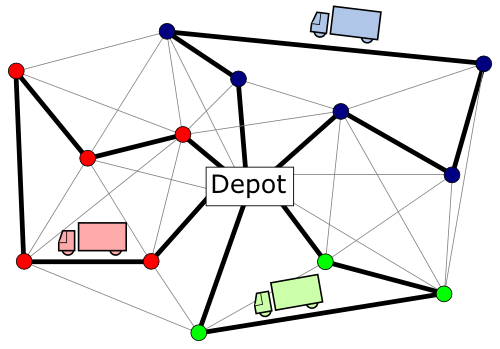
\includegraphics[width=40mm]{images/VRP.png}
      \end{column}
      \begin{column}{0.6\textwidth}
        \begin{itemize}
          \item Find optimal routes for multiple vehicles visiting a set of locations.
          \item 1 vehicle = Traveling Salesman Problem.
        \end{itemize}
      \end{column}
    \end{columns}
  \end{example}
\end{frame}

\begin{frame}
  \begin{example}[Vehicle routing]

    \begin{columns}
      \begin{column}{0.4\textwidth}        
        \centering
        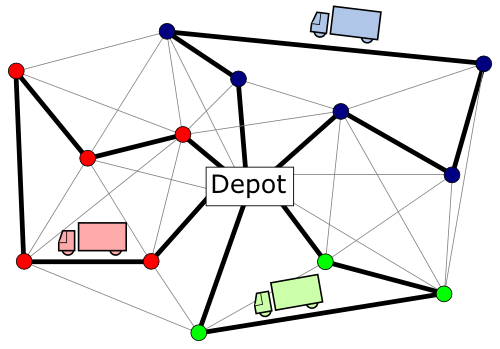
\includegraphics[width=40mm]{images/VRP.png} \\
      \end{column}
      \begin{column}{0.6\textwidth}        
        \begin{itemize}
          \item Find optimal routes for multiple vehicles visiting a set of locations
          \item 1 vehicle = Traveling Salesman Problem
        \end{itemize}
      \end{column}
    \end{columns}
  \end{example}

    Travelling salesman problem (generalise this for vehicle
    routing problems with multiple vehicles or with side constraints):

    \[
    \text{Circuit}(S)
    \]
    \[
    \text{Minimize} \quad \sum_{v=1}^{n} \text{distance}(v, S_v)
    \]   
\end{frame}

\begin{flashcardcpmpy}
\begin{frame}
  \begin{example}[Vehicle routing]

    \begin{columns}
      \begin{column}{0.4\textwidth}        
        \centering
        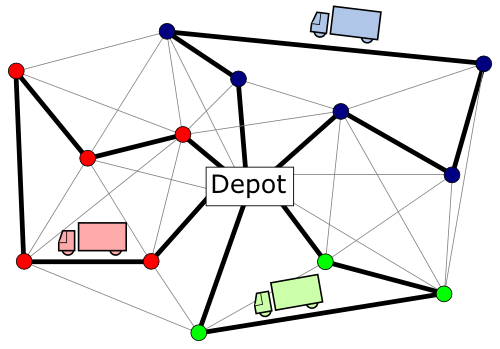
\includegraphics[width=40mm]{images/VRP.png} \\
      \end{column}
      \begin{column}{0.6\textwidth}        
        \begin{itemize}
          \item Find optimal routes for multiple vehicles visiting a set of locations
          \item 1 vehicle = Traveling Salesman Problem
        \end{itemize}
      \end{column}
    \end{columns}
  \end{example}

    Travelling salesman problem (generalise this for vehicle
    routing problems with multiple vehicles or with side constraints):

    \lstinputlisting[language=cpmpy,basicstyle=\small,firstline=14,lastline=15]{models_cpmpy/t4_circuit.py}

\end{frame}
\end{flashcardcpmpy}
\begin{flashcardminizinc}
\begin{frame}
  \begin{example}[Vehicle routing]

    \begin{columns}
      \begin{column}{0.4\textwidth}        
        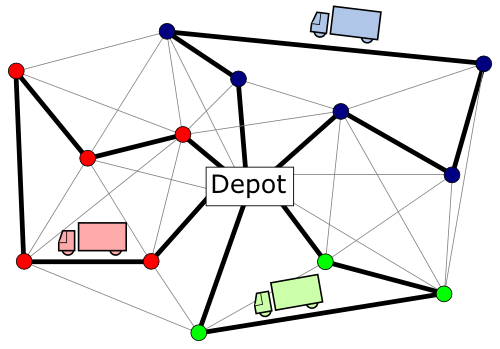
\includegraphics[width=60mm]{images/VRP.png} \\
      \end{column}
      \begin{column}{0.6\textwidth}        
        \begin{itemize}
          \item Find optimal routes for multiple vehicles visiting a set of locations
          \item 1 vehicle = Traveling Salesman Problem
        \end{itemize}
      \end{column}
    \end{columns}

    Travelling salesman problem (generalise this for vehicle
    routing problems with multiple vehicles or with side constraints):

    \vspace{-2mm}
    \lstinputlisting[language=Mzn,firstnumber=3,firstline=3,lastline=4]{models_minizinc/tsp.mzn}
    \vspace{-2mm}
    
    Requiring a \alert{directed path} from vertex \mzninline{v} to
    vertex \mzninline{w}: 
    \mzninline{constraint subcircuit(S) /\ S[w] = v;}
    upon adding \mzninline{v} to the domain of \mzninline{S[w]} if
    need be.
  \end{example}
  \vspace{-1mm}

  Many graph constraints, including \mzninline{dpath}, exist in
  \MiniZinc.
\end{frame}
\end{flashcardminizinc}


\subsection{\cons{Table}{}}

\begin{frame}
  \begin{definition}
    The \cons{Table}{X, T} constraint holds if and only if the values of the 1D array $X$ of decision variables form a row of the 2D array $T$ of values. In other words, it restricts the values of the given variables in $X$ to combinations listed in the predefined table $T$.
  \end{definition}
  \vfill
    
  The 2D array $T$ provides an \defined{extensional definition} of the constraint we impose. \\    
  Its decomposition is as follows:
  \[
  \exists \text{ row } \in T \text{ such that } \forall i, \, X_i = \text{row}_i
  \]
  \vfill
  
  \begin{example}
    Assigning Workers $W_1, W_2$ to Shifts, but only specific assignments are allowed:
    \[
    \text{T} = \{ (1, 2), (1, 3), (2, 3) \}
    \]

    The \cons{Table}{} constraint is applied as:
    \[
    \cons{Table}{[W_1, W_2], T}
    \]            
  \end{example}
\end{frame}

\begin{flashcardcpmpy}
\begin{frame}
  \begin{definition}
    The \cons{Table}{X, T} constraint holds if and only if the values of the 1D array $X$ of decision variables form a row of the 2D array $T$ of values. In other words, it restricts the values of the given variables in $X$ to combinations listed in the predefined table $T$.
  \end{definition}
  \vfill
    
  The 2D array $T$ provides an \defined{extensional definition} of the constraint we impose. \\    
  Its decomposition in \CPMpy is the following: \\
  \cpminline{[cp.any(cp.all(ai == ri for ai, ri in zip(arr, row)) for row in tab)]}
  \vfill

  \begin{example}
    Assigning Workers $W_1, W_2$ to Shifts, but only specific assignments are allowed:
    \lstinputlisting[language=cpmpy,numbers=none,basicstyle=\small,firstline=10,lastline=12]{models_cpmpy/t4_table.py}
  \end{example}
\end{frame}
\end{flashcardcpmpy}


\subsection{\cons{CountEq}{}}

\begin{frame}
  Given an array of decision variables $X$, we often want to count
  the number of decision variables in
  $X$ that are equal to a decision variable (or value) $val$.
  \vfill
  
  \begin{definition}[The \cons{CountEq}{} functional global constraint]
    The \cons{CountEq}{X, val, res} functional glboal constraint holds if and only if the number of occurrences of the numeric value/value of the variable $res$ in the array of decision variables $X$ is equal to $res$.
  \end{definition}\vfill
  
  Its decomposition is the following: \\
  \[
  \sum_{i}  [ X_i = v ]  = res
  \]
  \vfill

  \begin{example}[Unweighted Photo Alignment Problem]
    \begin{align*}
      \cons{CountEq}{\{ \left| \text{Pos}_{who} - \text{Pos}_{whom} \right| \mid (who, whom) \in \text{Wishes} \}, 1, res} \\
      \text{Maximize} \left( res \right)
    \end{align*}
  \end{example}
\end{frame}

\begin{flashcardcpmpy}
\begin{frame}
  Given an array of decision variables $X$, we often want to count
  the number of decision variables in
  $X$ that are equal to a decision variable (or value) $val$.
  \vfill
  
  \begin{definition}[The \cons{CountEq}{} functional global constraint]
    The \cons{CountEq}{X, val, res} functional glboal constraint holds if and only if the number of occurrences of the numeric value/value of the variable $res$ in the array of decision variables $X$ is equal to $res$.
  \end{definition}\vfill
  
  Its decomposition in \CPMpy is the following: \\
  \cpminline{res == cp.sum(X == val)}\vfill
  
  \begin{example}[Unweighted Photo Alignment Problem from L02]
    \cpminline{model +=} \\ \cpminline{  cp.Count([abs(Pos[who] - Pos[whom]) for (who,whom) in Wishes], 1) == res}
    \cpminline{model.maximize(res)}
  \end{example}
\end{frame}

\begin{frame}
  Given an array of decision variables $X$, we often want to count
  the number of decision variables in
  $X$ that are equal to a decision variable (or value) $val$.
  \vfill
  
  \begin{definition}[The \cons{CountEq}{} functional global constraint]
    The \cons{CountEq}{X, val, res} functional glboal constraint holds if and only if the number of occurrences of the numeric value/value of the variable $res$ in the array of decision variables $X$ is equal to $res$.
  \end{definition}\vfill
  
  Its decomposition in \CPMpy is the following: \\
  \cpminline{res == cp.sum(X == val)}\vfill
  
  \red{Functional formulation} (without explicit \texttt{res}):
  \begin{example}[Unweighted Photo Alignment Problem from L02]
    \cpminline{m.maximize(cp.Count([abs(Pos[who] - Pos[whom]) for (who,whom) in Wishes], 1))}
  \end{example}
\end{frame}
\end{flashcardcpmpy}

\begin{frame}{A Common Source of Inefficiency in Models}
  Group constraints in (more specific) globals when possible:
  \begin{example}
    The constraint specification
    \[
    \forall j \in \text{index\_set}(V), \; \text{CountEq}(X, V_j, C_j)
    \]
    should be reformulated, due to the \alert{shared} array $X$ for \alert{each} $j$, into: 
    \[
    \cons{GlobalCardinalityCount}{X, V, C}
    \]
    by applying the default definition backwards: \vfill
    \begin{itemize}
      \item At worst, it will be applied forward while decomposing;
      \item At best, the used solver will have better \inference{inference}.
    \end{itemize}
  \end{example}
\end{frame}

\begin{flashcardcpmpy}
\begin{frame}{A Common Source of Inefficiency in Models}
  Group constraints in (more specific) globals when possible:
  \begin{example}
    The constraint specification
    \begin{center}
      \cpminline{for v, c in zip(V, C): cp.Count(X, v) == c} 
    \end{center}\vfill
    should be reformulated, due to the \alert{shared} array $X$ for \alert{each} $j$, into: 
    \begin{center}
      \cpminline{cp.GlobalCardinalityCount(X,V,C);}
    \end{center}\vfill
    by applying the default definition backwards: \vfill
    \begin{itemize}
      \item At worst, it will be applied forward while decomposing;
      \item At best, the used solver will have better \inference{inference}.
    \end{itemize}
  \end{example}
\end{frame}
\end{flashcardcpmpy}

    
\subsection{\cons{NvalueEq}{}}

\begin{frame}
  \begin{definition}[Pachet and Roy, 1999]
    The \cons{NvalueEq}{X, res} functional global constraint holds if and only if the number of distinct values taken by the elements of the array $X$ of decision variables is equal to $res$. If array $X$ is 1d, with length $n$, then this means:
    \[
      \Cardinality{\Set{X_0,\dots,X_{n-1}}}
    \]
  \end{definition}
  \vfill

  If $\Cardinality{X} = n$ then \cons{NvalueEq}{X, n} means \cons{AllDifferent}{X}, \\
  but: \alert{always use the most specific available constraint predicate!}
  \vfill

  \begin{example}
    Graph colouring: Different colour on neighbouring nodes + minimize the number of colours, i.e., minimize the number of \emph{distinct} values of our variables:
    \begin{align*}        
      &\text{node}_{1} \neq \text{node}_{2}, &\forall (\text{node}_1, \text{node}_2) \in \text{Edges} \\
      &\cons{NvalueEq}{\text{nodes}, res} &\\
      &\minimize res &
    \end{align*}
  \end{example}
\end{frame}

\begin{flashcardcpmpy}
\begin{frame}
  \begin{definition}[Pachet and Roy, 1999]
    The \cons{NvalueEq}{X, res} functional global constraint holds if and only if the number of distinct values taken by the elements of the array $X$ of decision variables is equal to $res$. If array $X$ is 1d, with length $n$, then this means:
    \[
      \Cardinality{\Set{X_0,\dots,X_{n-1}}}
    \]
  \end{definition}
  \vfill

  If $\Cardinality{X} = n$ then \cons{NvalueEq}{X, n} means \cons{AllDifferent}{X}, \\
  but: \alert{always use the most specific available constraint predicate!}
  \vfill

  \begin{example}
    Graph colouring: Different colour on neighbouring nodes + minimize the number of colours, i.e., minimize the number of \emph{distinct} values of our variables:
    \lstinputlisting[language=cpmpy,basicstyle=\small,firstline=12,lastline=15]{models_cpmpy/t4_nvalue.py}
  \end{example}
\end{frame}
\end{flashcardcpmpy}


\subsection{\cons{ElementEq}{}}

\begin{frame}
  Modeling an \textcolor{Melon}{unknown element of an array}.
  \vfill

  \begin{example}[Job allocation at minimal salary cost]
    \structured{Given} the salaries of work applicants $Salary$ for different jobs, \\
    \structured{find} a work applicant
    for each job \structured{such that} some constraints (on the
    qualifications of the work applicants for the jobs, on workload
    distribution, etc) are satisfied and the \textbf{total salary cost is
    minimal}: 

    \begin{align*}
      &\text{total\_cost} = \sum_{ w \in \text{workers}} \text{Salary}_{w}\\
      &\minimize \text{total\_cost}
    \end{align*}
    
    \vfill
    \alert{We do not know at modelling time the worker allocated to each job!}
  \end{example}
\end{frame}

\begin{flashcardcpmpy}
\begin{frame}
  Modeling an \textcolor{Melon}{unknown element of an array}.
  \vfill

  \begin{example}[Job allocation at minimal salary cost]
    \structured{Given} the salaries of work applicants $Salary$ for different jobs, \\
    \structured{find} a work applicant
    for each job \structured{such that} some constraints (on the
    qualifications of the work applicants for the jobs, on workload
    distribution, etc) are satisfied and the \textbf{total salary cost is
    minimal}: 
    \vfill

    \lstinputlisting[language=cpmpy,basicstyle=\footnotesize,firstline=17,lastline=20,numbers=none]{models_cpmpy/t4_element.py} \vfill
    %Line~3 is equivalent to the less readable formulation: \\
    %\cpminline{total_cost = cp.sum([cp.Element(Salary, worker) for worker in workers])}
    \vfill

    \alert{We do not know at modelling time the worker allocated to each job!} \\ \vfill
    We need to express the relation between variables/expressions and values of arrays based on unknown indices \dots
  \end{example}
\end{frame}
\end{flashcardcpmpy}

\begin{frame}{The \cons{ElementEq}{} Global Constraint}
  We need to express the the relation between variables/expressions and values of arrays based on unknown indices \dots

  \begin{definition}[Van Hentenryck and Carillon, 1988]
    The \cons{ElementEq}{Arr, idx, res} functional global constraint holds if and only if the value $Arr[idx] = res$, where $Arr$ is array of decision variables or constants and $idx$ is an integer \alert{decision variable}.
  \end{definition}\vfill
  
  \alert{For better model readability}, the \cons{ElementEq}{} predicate is typically not directly used,
  when modeling languages allow direct indexing; e.g. \texttt{res == Arr[idx]}
  even if \texttt{idx} is an integer expression involving at least one decision variable.
  \vfill

  Note that \cons{Element}{} can be multi-dimensional: \cpminline{Arr[idx1, idx2]}
  We assume that the indices can only take values \alert{within the bounds of the array.}
\end{frame}


\begin{frame}{Summary}
  Global Constraints:
  \begin{itemize}
    \item Non-fixed arity
    \item Model global properties of the problem
  \end{itemize}
  \vfill

  \textbf{Building blocks} that can be used in modeling a variety of problems \dots
  \begin{itemize}
    \item \textit{Expressiveness}!! Closer to problem definition
  \end{itemize}
  \vfill

  \textbf{Better inference} during solving \dots ~\textit{Efficiency}!!
  \begin{itemize}
    \item Due to modeling global properties together
    \item Potentially fewer auxiliary variables
    \item Potentially more effective propagators
  \end{itemize}
\end{frame}

\end{document}
